% ============================================================
% Question Bank: ch07-02 Circumference of a Circle
% Topic Title: Circumference of a Circle
% CCSS: 7.G.B.4
% Questions: 27 (15 MC + 6 SA + 6 Graphical)
% ============================================================

% --- Multiple Choice Questions (15) ---

\begin{practiceQuestion}{7-2-q01}{mc}
\begin{questionText}
What is the circumference of a circle with a diameter of $7$ cm? Use $\pi \approx \frac{22}{7}$.
\end{questionText}
\choiceA{$11$ cm}
\choiceB{$22$ cm}
\choiceC{$44$ cm}
\choiceD{$154$ cm}
\correctAnswer{B}
\explanation{The circumference formula is $C = \pi d$. Substituting: $C = \frac{22}{7} \times 7 = 22$ cm.}
\end{practiceQuestion}

\begin{practiceQuestion}{7-2-q02}{mc}
\begin{questionText}
What is the circumference of a circle with a radius of $9$ inches? Use $\pi \approx 3.14$.
\end{questionText}
\choiceA{$28.26$ in}
\choiceB{$56.52$ in}
\choiceC{$113.04$ in}
\choiceD{$254.34$ in}
\correctAnswer{B}
\explanation{The circumference formula using radius is $C = 2\pi r$. Substituting: $C = 2 \times 3.14 \times 9 = 56.52$ inches.}
\end{practiceQuestion}

\begin{practiceQuestion}{7-2-q03}{mc}
\begin{questionText}
Which formula gives the circumference of a circle when the diameter is known?
\end{questionText}
\choiceA{$C = \pi r$}
\choiceB{$C = \pi d$}
\choiceC{$C = \pi r^2$}
\choiceD{$C = 2\pi d$}
\correctAnswer{B}
\explanation{When the diameter is known, use $C = \pi d$. The alternative formula $C = 2\pi r$ is used when the radius is known.}
\end{practiceQuestion}

\begin{practiceQuestion}{7-2-q04}{mc}
\begin{questionText}
A circle has a circumference of $37.68$ cm. Using $\pi \approx 3.14$, what is its diameter?
\end{questionText}
\choiceA{$6$ cm}
\choiceB{$12$ cm}
\choiceC{$24$ cm}
\choiceD{$118.30$ cm}
\correctAnswer{B}
\explanation{Rearrange $C = \pi d$ to get $d = C \div \pi = 37.68 \div 3.14 = 12$ cm.}
\end{practiceQuestion}

\begin{practiceQuestion}{7-2-q05}{mc}
\begin{questionText}
A circular running track has a radius of $25$ meters. What is the distance around one lap? Use $\pi \approx 3.14$.
\end{questionText}
\choiceA{$78.5$ m}
\choiceB{$157$ m}
\choiceC{$314$ m}
\choiceD{$1{,}962.5$ m}
\correctAnswer{B}
\explanation{The distance around the track is the circumference: $C = 2\pi r = 2 \times 3.14 \times 25 = 157$ meters.}
\end{practiceQuestion}

\begin{practiceQuestion}{7-2-q06}{mc}
\begin{questionText}
A coin has a diameter of $2$ cm. How far does it roll in one complete turn? Use $\pi \approx 3.14$.
\end{questionText}
\choiceA{$1.57$ cm}
\choiceB{$3.14$ cm}
\choiceC{$6.28$ cm}
\choiceD{$12.56$ cm}
\correctAnswer{C}
\explanation{In one complete turn, the coin rolls a distance equal to its circumference: $C = \pi d = 3.14 \times 2 = 6.28$ cm.}
\end{practiceQuestion}

\begin{practiceQuestion}{7-2-q07}{mc}
\begin{questionText}
A circular swimming pool has a circumference of $47.1$ feet. Using $\pi \approx 3.14$, what is the radius of the pool?
\end{questionText}
\choiceA{$7.5$ feet}
\choiceB{$15$ feet}
\choiceC{$23.55$ feet}
\choiceD{$30$ feet}
\correctAnswer{A}
\explanation{First find the diameter: $d = C \div \pi = 47.1 \div 3.14 = 15$ feet. Then the radius is $r = d \div 2 = 15 \div 2 = 7.5$ feet.}
\end{practiceQuestion}

\begin{practiceQuestion}{7-2-q08}{mc}
\begin{questionText}
A tractor tire has a diameter of $24$ inches. How far does it travel in one full rotation? Use $\pi \approx 3.14$.
\end{questionText}
\choiceA{$37.68$ in}
\choiceB{$75.36$ in}
\choiceC{$150.72$ in}
\choiceD{$452.16$ in}
\correctAnswer{B}
\explanation{One full rotation covers the circumference: $C = \pi d = 3.14 \times 24 = 75.36$ inches.}
\end{practiceQuestion}

\begin{practiceQuestion}{7-2-q09}{mc}
\begin{questionText}
If you double the diameter of a circle, what happens to its circumference?
\end{questionText}
\choiceA{It stays the same.}
\choiceB{It doubles.}
\choiceC{It triples.}
\choiceD{It quadruples.}
\correctAnswer{B}
\explanation{Since $C = \pi d$, the circumference is directly proportional to the diameter. If $d$ doubles, then $C$ also doubles.}
\end{practiceQuestion}

\begin{practiceQuestion}{7-2-q10}{mc}
\begin{questionText}
The minute hand of a clock is $6$ inches long. What distance does the tip of the minute hand travel in one full revolution? Use $\pi \approx 3.14$.
\end{questionText}
\choiceA{$18.84$ in}
\choiceB{$37.68$ in}
\choiceC{$75.36$ in}
\choiceD{$113.04$ in}
\correctAnswer{B}
\explanation{The tip traces a circle with radius $6$ inches. The circumference is $C = 2\pi r = 2 \times 3.14 \times 6 = 37.68$ inches.}
\end{practiceQuestion}

\begin{practiceQuestion}{7-2-q11}{mc}
\begin{questionText}
A hula hoop has a diameter of $3$ feet. What is its circumference? Use $\pi \approx 3.14$.
\end{questionText}
\choiceA{$4.71$ ft}
\choiceB{$6.28$ ft}
\choiceC{$9.42$ ft}
\choiceD{$18.84$ ft}
\correctAnswer{C}
\explanation{The circumference is $C = \pi d = 3.14 \times 3 = 9.42$ feet.}
\end{practiceQuestion}

\begin{practiceQuestion}{7-2-q12}{mc}
\begin{questionText}
A circular mirror has a radius of $10$ cm. What is its circumference? Use $\pi \approx 3.14$.
\end{questionText}
\choiceA{$31.4$ cm}
\choiceB{$62.8$ cm}
\choiceC{$125.6$ cm}
\choiceD{$314$ cm}
\correctAnswer{B}
\explanation{The circumference is $C = 2\pi r = 2 \times 3.14 \times 10 = 62.8$ cm.}
\end{practiceQuestion}

\begin{practiceQuestion}{7-2-q13}{mc}
\begin{questionText}
Circle A has a circumference of $31.4$ cm and Circle B has a circumference of $62.8$ cm. Using $\pi \approx 3.14$, how do their diameters compare?
\end{questionText}
\choiceA{Circle B's diameter is half of Circle A's.}
\choiceB{Their diameters are equal.}
\choiceC{Circle B's diameter is twice Circle A's.}
\choiceD{Circle B's diameter is four times Circle A's.}
\correctAnswer{C}
\explanation{$d_A = 31.4 \div 3.14 = 10$ cm. $d_B = 62.8 \div 3.14 = 20$ cm. Circle B's diameter is twice Circle A's because circumference is proportional to diameter.}
\end{practiceQuestion}

\begin{practiceQuestion}{7-2-q14}{mc}
\begin{questionText}
A roll of tape has a diameter of $3.5$ inches. What is the circumference of the roll? Use $\pi \approx 3.14$.
\end{questionText}
\choiceA{$5.50$ in}
\choiceB{$10.99$ in}
\choiceC{$21.98$ in}
\choiceD{$38.47$ in}
\correctAnswer{B}
\explanation{The circumference is $C = \pi d = 3.14 \times 3.5 = 10.99$ inches.}
\end{practiceQuestion}

\begin{practiceQuestion}{7-2-q15}{mc}
\begin{questionText}
A piece of string that is exactly $18.84$ cm long is formed into a circle. Using $\pi \approx 3.14$, what is the radius of the circle?
\end{questionText}
\choiceA{$3$ cm}
\choiceB{$6$ cm}
\choiceC{$9$ cm}
\choiceD{$12$ cm}
\correctAnswer{A}
\explanation{The string length is the circumference. Use $C = 2\pi r$ to find $r = C \div (2\pi) = 18.84 \div 6.28 = 3$ cm.}
\end{practiceQuestion}

% --- Short Answer Questions (6) ---

\begin{practiceQuestion}{7-2-q16}{sa}
\begin{questionText}
A circular fountain has a diameter of $15$ feet. What is its circumference? Use $\pi \approx 3.14$.
\end{questionText}
\correctAnswer{$47.1$ feet}
\explanation{The circumference is $C = \pi d = 3.14 \times 15 = 47.1$ feet.}
\end{practiceQuestion}

\begin{practiceQuestion}{7-2-q17}{sa}
\begin{questionText}
A circular garden has a radius of $11$ meters. What is the circumference? Use $\pi \approx 3.14$.
\end{questionText}
\correctAnswer{$69.08$ meters}
\explanation{The circumference is $C = 2\pi r = 2 \times 3.14 \times 11 = 69.08$ meters.}
\end{practiceQuestion}

\begin{practiceQuestion}{7-2-q18}{sa}
\begin{questionText}
A circle has a circumference of $50.24$ cm. Using $\pi \approx 3.14$, what is the radius?
\end{questionText}
\correctAnswer{$8$ cm}
\explanation{First find the diameter: $d = C \div \pi = 50.24 \div 3.14 = 16$ cm. Then the radius is $r = 16 \div 2 = 8$ cm.}
\end{practiceQuestion}

\begin{practiceQuestion}{7-2-q19}{sa}
\begin{questionText}
A wall clock has a diameter of $12$ inches. What is the circumference of the clock? Use $\pi \approx 3.14$.
\end{questionText}
\correctAnswer{$37.68$ inches}
\explanation{The circumference is $C = \pi d = 3.14 \times 12 = 37.68$ inches.}
\end{practiceQuestion}

\begin{practiceQuestion}{7-2-q20}{sa}
\begin{questionText}
Two circles have radii of $5$ cm and $10$ cm. What is the difference in their circumferences? Use $\pi \approx 3.14$.
\end{questionText}
\correctAnswer{$31.4$ cm}
\explanation{$C_1 = 2 \times 3.14 \times 5 = 31.4$ cm. $C_2 = 2 \times 3.14 \times 10 = 62.8$ cm. The difference is $62.8 - 31.4 = 31.4$ cm.}
\end{practiceQuestion}

\begin{practiceQuestion}{7-2-q21}{sa}
\begin{questionText}
A bicycle wheel has a radius of $14$ inches. How far does the wheel travel in one full rotation? Use $\pi \approx \frac{22}{7}$.
\end{questionText}
\correctAnswer{$88$ inches}
\explanation{The wheel travels one circumference per rotation: $C = 2\pi r = 2 \times \frac{22}{7} \times 14 = 2 \times 44 = 88$ inches.}
\end{practiceQuestion}

% --- Graphical Questions (3 GMC + 3 GSA) ---

\begin{practiceQuestion}{7-2-q22}{gmc}
\begin{questionText}
The circle below has a diameter labeled. What is the circumference of the circle? Use $\pi \approx 3.14$.

\begin{center}
\begin{tikzpicture}
  \draw[thick] (0,0) circle (2);
  \fill (0,0) circle (2pt) node[below] {$O$};
  \draw[thick,funBlue] (-2,0) -- (2,0) node[midway,above] {$d = 12$ cm};
  \fill (-2,0) circle (2pt);
  \fill (2,0) circle (2pt);
\end{tikzpicture}
\end{center}
\end{questionText}
\choiceA{$18.84$ cm}
\choiceB{$37.68$ cm}
\choiceC{$75.36$ cm}
\choiceD{$452.16$ cm}
\correctAnswer{B}
\explanation{The circumference is $C = \pi d = 3.14 \times 12 = 37.68$ cm.}
\end{practiceQuestion}

\begin{practiceQuestion}{7-2-q23}{gmc}
\begin{questionText}
The circle below has a radius labeled. What is the circumference of the circle? Use $\pi \approx 3.14$.

\begin{center}
\begin{tikzpicture}
  \draw[thick] (0,0) circle (2);
  \fill (0,0) circle (2pt) node[below left] {$O$};
  \draw[thick,funBlue] (0,0) -- (1.41,1.41) node[midway,below right] {$r = 5$ cm};
  \fill (1.41,1.41) circle (2pt);
\end{tikzpicture}
\end{center}
\end{questionText}
\choiceA{$15.7$ cm}
\choiceB{$31.4$ cm}
\choiceC{$62.8$ cm}
\choiceD{$78.5$ cm}
\correctAnswer{B}
\explanation{The circumference is $C = 2\pi r = 2 \times 3.14 \times 5 = 31.4$ cm.}
\end{practiceQuestion}

\begin{practiceQuestion}{7-2-q24}{gmc}
\begin{questionText}
The semicircle below has a diameter of $10$ cm. What is the perimeter of the entire semicircular shape (the curved part plus the straight edge)? Use $\pi \approx 3.14$.

\begin{center}
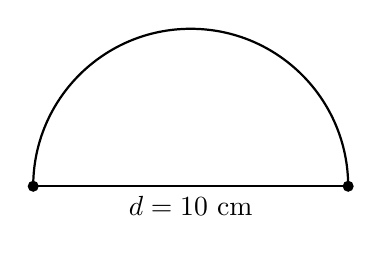
\begin{tikzpicture}
  \draw[thick] (2,0) arc (0:180:2);
  \draw[thick] (-2,0) -- (2,0) node[midway,below] {$d = 10$ cm};
  \fill (-2,0) circle (2pt);
  \fill (2,0) circle (2pt);
\end{tikzpicture}
\end{center}
\end{questionText}
\choiceA{$15.7$ cm}
\choiceB{$25.7$ cm}
\choiceC{$31.4$ cm}
\choiceD{$41.4$ cm}
\correctAnswer{B}
\explanation{The curved part is half the circumference: $\frac{1}{2} \times \pi d = \frac{1}{2} \times 3.14 \times 10 = 15.7$ cm. Add the straight edge: $15.7 + 10 = 25.7$ cm.}
\end{practiceQuestion}

\begin{practiceQuestion}{7-2-q25}{gsa}
\begin{questionText}
The circle below has a radius labeled. Find the circumference. Use $\pi \approx 3.14$.

\begin{center}
\begin{tikzpicture}
  \draw[thick] (0,0) circle (2);
  \fill (0,0) circle (2pt) node[below left] {$O$};
  \draw[thick,funBlue] (0,0) -- (2,0) node[midway,below] {$r = 6$ cm};
  \fill (2,0) circle (2pt);
\end{tikzpicture}
\end{center}
\end{questionText}
\correctAnswer{$37.68$ cm}
\explanation{The circumference is $C = 2\pi r = 2 \times 3.14 \times 6 = 37.68$ cm.}
\end{practiceQuestion}

\begin{practiceQuestion}{7-2-q26}{gsa}
\begin{questionText}
The circle below has a diameter labeled. Find the circumference. Use $\pi \approx 3.14$.

\begin{center}
\begin{tikzpicture}
  \draw[thick] (0,0) circle (2.2);
  \fill (0,0) circle (2pt) node[below] {$O$};
  \draw[thick,funBlue] (-2.2,0) -- (2.2,0) node[midway,above] {$d = 18$ cm};
  \fill (-2.2,0) circle (2pt);
  \fill (2.2,0) circle (2pt);
\end{tikzpicture}
\end{center}
\end{questionText}
\correctAnswer{$56.52$ cm}
\explanation{The circumference is $C = \pi d = 3.14 \times 18 = 56.52$ cm.}
\end{practiceQuestion}

\begin{practiceQuestion}{7-2-q27}{gsa}
\begin{questionText}
Two concentric circles are shown below. How much farther would you walk around the outer circle than around the inner circle? Use $\pi \approx 3.14$.

\begin{center}
\begin{tikzpicture}
  \draw[thick,funBlue] (0,0) circle (2.5);
  \draw[thick,funOrange] (0,0) circle (1);
  \fill (0,0) circle (2pt) node[below left] {$O$};
  \draw[thick,funBlue,->] (0,0) -- (2.5,0) node[midway,above] {$7$};
  \draw[thick,funOrange,->] (0,0) -- (0,-1) node[midway,right] {$3$};
\end{tikzpicture}
\end{center}
\end{questionText}
\correctAnswer{$25.12$ units}
\explanation{Outer circumference: $C = 2 \times 3.14 \times 7 = 43.96$. Inner circumference: $C = 2 \times 3.14 \times 3 = 18.84$. Difference: $43.96 - 18.84 = 25.12$ units.}
\end{practiceQuestion}
